\documentclass[journal]{IEEEtran}

\usepackage{amsmath,amssymb,amsfonts}
\usepackage{graphicx}
\usepackage{booktabs}
\usepackage{multirow}
\usepackage{array}
\usepackage{makecell}
\usepackage{microtype}
\usepackage{cite}
\usepackage{url}
\usepackage[hidelinks]{hyperref}

\newcommand{\sys}{AAFV-Net}
\newcommand{\vect}[1]{\mathbf{#1}}

\begin{document}

\title{AAFV-Net: Guarded Three-Way Age-Aware Face Verification With Empirically Bounded Random False-Accept Risk}

% NOTE FOR SUBMISSION: Replace bracketed placeholders below with complete verified co-author names,
% institutional affiliations, city/country, grants, and ORCID iDs (via \orcidlink if supported).
\author{Anurag~Nayak,~\IEEEmembership{Graduate Student Member,~IEEE,}
        [Co-Author~Names~To~Be~Completed]%
\thanks{Manuscript submitted November 12, 2026. [Add verified grant/funding sponsorship or state no external funding received.]}%
\thanks{A.~Nayak and [Co-Authors] are with the [Department, University/Institution Name, City, State/Postal Code, Country] (e-mail: contact@anuragnayak.dev; ORCID: [0000-0000-0000-0000]). Code, frozen model checksums, and access logs are available at \url{https://github.com/anuragnayak01/AAFV_Net}.}}

\markboth{Submitted to IEEE Transactions on Information Forensics and Security}%
{Nayak \MakeLowercase{\textit{et al.}}: AAFV-Net: Guarded Three-Way Age-Aware Face Verification}

\maketitle

\begin{abstract}
Verifying facial identity across multi-year age gaps remains challenging in operational security workflows where admitting an impostor incurs severe consequences. Conventional single-threshold matchers optimize ranking metrics such as area under the curve, yet fail to bound false-accept rates on frozen deployment operating points when age drift and look-alike impostors overlap. We present AAFV-Net, an adult cross-age face verification framework formulated as a guarded three-way decision rule partitioning pairs into auto-accept, manual review, and auto-reject zones. For each pair, AAFV-Net combines five direct perceptual and identity similarities with bidirectional and five-year grid shared-target counterfactual progressions generated by Style-based Age Manipulation, fused through a 947-parameter ensemble perceptron with stochastic branch masking, explicit face quality, synthesis reliability, and normalized age-gap context. Decision thresholds are frozen under SHA-256 checksums on sequestered calibration splits before testing under a logged two-look budget. On person-disjoint MORPH test pairs, AAFV-Net records zero false accepts across 1,149 same-sex bipartite random impostors, yielding a 0.320 percent one-sided 95 percent upper bound under two-look Bonferroni adjustment, while accepting 70.07 percent of 24,305 genuine pairs and rejecting 98.04 percent of 35,735 hard impostors (with five residual hard false accepts) and 57.49 percent of neutral hard impostors. Evaluated zero-shot on external FG-NET adult pairs (ages 16 and older), AAFV-Net raises auto-accept from 40.38 percent to 51.92 percent over ArcFace with zero impostor false accepts.
\end{abstract}

\begin{IEEEkeywords}
Biometric security, calibration, confidence bounds, cross-age face verification, generative age synthesis, reject option, three-way decision.
\end{IEEEkeywords}

\section{Introduction}
\label{sec:intro}
\IEEEPARstart{C}{ross-age} facial verification underpins automated border control, identity credential renewal, forensic image comparison, and missing-persons investigations~\cite{grother2019frvt_part3,bestrowden2018longitudinal}. Across spans ranging from years to decades, craniofacial aging produces epidermal texture changes, soft-tissue redistribution, and skeletal remodeling that inflate intra-subject embedding dispersion~\cite{lanitis2002fgnet,bestrowden2018longitudinal}. Under strict high-security operating points, deep angular-margin matchers such as ArcFace~\cite{deng2019arcface} face a structural dilemma: tightening decision thresholds to suppress impostors rejects genuine longitudinal matches, whereas loosening thresholds exposes the system to look-alike false accepts~\cite{paone2014twins}.

Conventional biometric verification pipelines force a binary accept/reject outcome from a single threshold~$T$ and report dataset-wide ranking statistics such as Area Under the Curve (AUC) or True Match Rate at a fixed nominal False Match Rate (FMR)~\cite{otroshi2024inversion}. As illustrated in Fig.~\ref{fig:concept}(a), single-threshold matchers suffer two interrelated vulnerabilities in high-assurance deployments:
\begin{enumerate}
    \item \textbf{Uncontained Ambiguity Exposure:} Genuine cross-age pairs experiencing biometric drift overlap in score space with near-threshold hard impostors; any binary threshold either admits look-alike impostors or discards authentic matches without structured escalation.
    \item \textbf{Misalignment Between Ranking AUC and Zero-Failure Thresholds:} Even deep classifiers with high aggregate AUC can produce heavy calibration impostor score tails~\cite{xu2024asc}, forcing a minimax zero-calibration-FA accept cutoff near~$1.0$ where virtually no genuine pair is accepted.
\end{enumerate}

\begin{figure}[t]
\centering
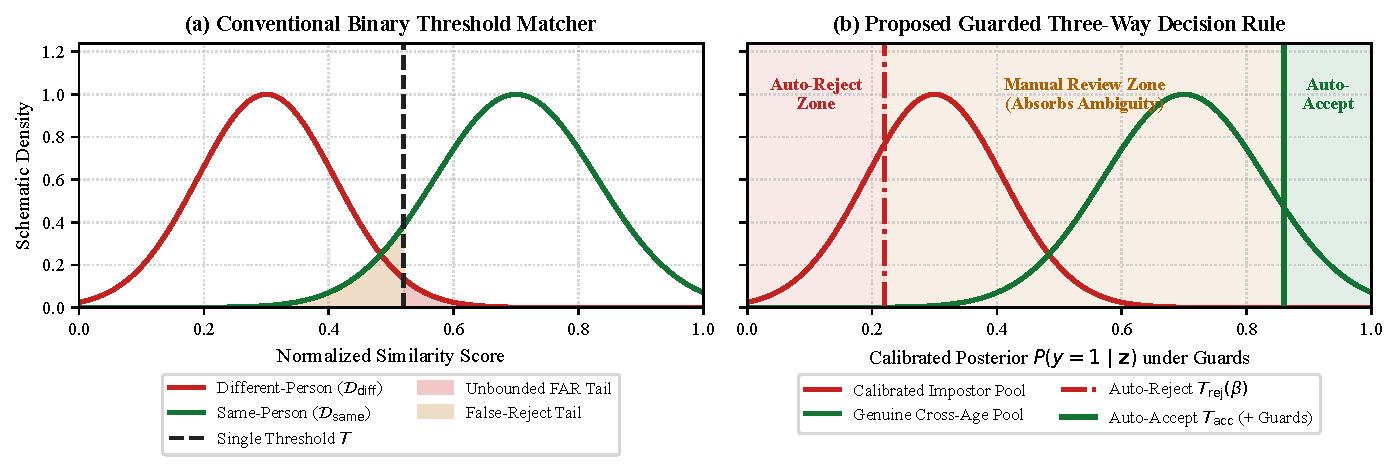
\includegraphics[width=\columnwidth]{figures/fig1_concept.pdf}
\caption{Decision topology comparison. (a)~Conventional binary threshold matchers expose uncontained tail overlaps between drifted genuine pairs and hard impostors. (b)~\sys\ maps pairs to calibrated posteriors subject to quality, reliability, and branch probability guards, separating high-confidence accepts ($T_{\text{acc}}$) and calibrated $\beta$-budget rejects ($T_{\text{rej}}(\beta)$) via an explicit manual-review zone.}
\label{fig:concept}
\end{figure}

To isolate uncertainty systematically, we formulate cross-age facial verification as a guarded, three-way classification problem inspired by Chow's reject-option framework~\cite{chow1970reject} and Neyman-Pearson hypothesis testing~\cite{hu2025neyman}. Rather than forcing every pair into a binary verdict, \sys\ routes pairs across three mutually exclusive operational regions (Fig.~\ref{fig:concept}(b)):
\begin{itemize}
    \item \textbf{Auto-Accept:} High-confidence adult pairs exceeding a frozen threshold~$T_{\text{acc}}$ and satisfying explicit input quality, synthesis reliability, and branch-level probability guards.
    \item \textbf{Manual Review:} Ambiguous, low-quality, or guard-failing pairs escalated to human examiners, containing tail overlap rather than forcing risky autonomous decisions.
    \item \textbf{Auto-Reject:} Clear mismatches below a quantile threshold~$T_{\text{rej}}(\beta)$ calibrated to control the training-free false-reject budget~$\beta$.
\end{itemize}

\sys\ couples direct multi-metric visual evidence with synthetic aging counterfactuals generated by the Style-based Age Manipulation (SAM) network~\cite{alaluf2021sam}. Crucially, rather than trusting synthesized faces as identity-preserving replacements~\cite{zhou2024openset}, \sys\ treats SAM as an auxiliary noisy channel whose output is quality-scored, trained under stochastic branch masking~\cite{poh2009quality}, and gated at inference. All parameters and thresholds are SHA-256 sealed prior to protected test evaluation under a strictly logged two-look budget.

\textbf{Contributions:} This work makes four verifiable contributions scoped to adult cross-age verification ($a \ge 16$):
\begin{enumerate}
    \item \textbf{Guarded Three-Way Decision Architecture:} We pair a direct five-metric evidence branch with a hedged counterfactual SAM aging branch through a lightweight 947-parameter fusion MLP, Platt calibration, branch probability guards, and empirical quality/reliability floors.
    \item \textbf{Empirical Resolution of Minimax Threshold Collapse:} Under an identical zero-calibration-FA accept rule, uncalibrated deep baselines (Siamese CNN, Siamese ViT, LoRA-adapted Qwen2-VL-2B) collapse to $\le 0.21\%$ auto-accept and single-branch ArcFace rejects $0.00\%$ of hard impostors, whereas \sys\ sustains $70.07\%$ same-person acceptance alongside $98.04\%$ hard-impostor and $57.49\%$ model-neutral hard-impostor rejection.
    \item \textbf{Scoped Statistical Risk Auditing:} Using within-sex bipartite person-disjoint random sampling ($\mathcal{D}_{\text{random}}, N=1{,}149$), pre-registered SHA-256 artifacts, and two-look Bonferroni accounting, \sys\ establishes an analytical 95\% upper bound of $0.320\%$ on random impostor FAR while transparently reporting empirical residual look-alike errors ($5/35{,}735$ on $\mathcal{D}_{\text{hard}}$) and abstaining from invalid i.i.d.\ claims on correlated pools.
    \item \textbf{External Generalization, Fairness, and Negative-Result Transparency:} Evaluated without retraining on FG-NET adults, \sys\ improves auto-accept across all six age-gap strata ($51.92\%$ vs.\ $40.38\%$ for ArcFace, $0/3{,}670$ impostor FAs), while explicitly characterizing pediatric failure ($4/20{,}000$ FAs under age 16), MORPH extreme-gap degradation, and a $9.14$ percentage-point sex acceptance disparity observed in Look~1.
\end{enumerate}

\section{Related Work}
\label{sec:related}
We organize closely related research into five thematic threads bridging face biometrics, generative synthesis skepticism, multimodal fusion calibration, bounded statistical testing, and fairness.

\subsection{Cross-Age and Age-Invariant Face Recognition}
Discriminative age-invariant face recognition (AIFR) models aim to purge age covariates from identity representations. Early subspace approaches~\cite{li2011aifr} evolved into deep orthogonal decomposition (OE-CNN)~\cite{wang2018oecnn}, decorrelated adversarial learning (DAL)~\cite{wang2019dal}, multi-task identity-disentangled frameworks (MTLFace)~\cite{huang2021mtlface}, and order-enhanced ordinal contrastive learning (OrdCon)~\cite{wang2025ordcon}. Longitudinal covariate studies~\cite{bestrowden2018longitudinal} nonetheless confirm that genuine similarity decays over multi-decade lapses even in strong angular-margin matchers such as CosFace~\cite{wang2018cosface} and ArcFace~\cite{deng2019arcface}. Conversely, privacy-funnel encoders~\cite{razeghi2026privacy} deliberately suppress soft biometric attributes including age. Unlike embedding-purging approaches, \sys\ leaves frozen identity extractors intact and preserves normalized age span~$g$ as an explicit context signal weighting direct versus synthesized evidence.

\subsection{Generative Face Aging and Forensic Counterfactuals}
Conditional aging generators progressed from adversarial autoencoders (CAAE)~\cite{zhang2017caae} and identity-preserving conditional GANs (IPCGANs)~\cite{tang2018ipcgan} to progressive sub-network chaining (PFA-GAN)~\cite{huang2021pfagan} and StyleGAN2 $\mathcal{W}+$ latent age regression (SAM)~\cite{alaluf2021sam,karras2020stylegan2}. However, forensic open-set studies~\cite{zhou2024openset} highlight that synthetic face generators suffer semantic artifacts and identity drift under domain shifts or extreme structural change (such as early childhood growth). \sys\ avoids treating SAM syntheses as ground-truth faces; instead, it summarizes five-year snapped grid counterfactuals via z-standardized mean pooling, scores per-synthesis reliability~$R_{\text{sam}}$, and trains under $p_{\text{mask}}=0.12$ branch masking so inference never depends unconditionally on generative synthesis.

\subsection{Quality-Dependent Multimodal Fusion and Calibration}
Score-level fusion and quality conditioning provide essential precursors to \sys. Poh \emph{et al.}~\cite{poh2009quality} benchmarked quality-dependent multimodal score fusion and explicit missing-channel dropout across biometric modalities, establishing how auxiliary-channel unreliability degrades unguarded linear combiners. Recent face verification studies confirm that angular cosine scores exhibit miscalibration under cross-age noise and look-alikes: Xu \emph{et al.}~\cite{xu2024asc} introduced Angular Scaling Calibration (ASC) to minimize expected calibration error, and Ahn \emph{et al.}~\cite{ahn2024ucface} learned quality-conditioned probabilistic embeddings (UCFace) for open-set rejection. While complementary, ASC optimizes unguarded single-branch calibration and UCFace requires retraining backbone extractors. \sys\ adapts Poh \emph{et al.}'s quality-weighted missing-channel paradigm to frozen multi-metric similarity vectors (ArcFace, EfficientNet-B0~\cite{tan2019efficientnet}, VGG-Face~\cite{parkhi2015vgg}, LPIPS~\cite{zhang2018lpips}, SSIM~\cite{wang2004ssim}) via Platt scaling~\cite{platt1999} and explicit probability/quality guards.

\subsection{Reject-Option Classification and Finite-Sample Bounds}
Chow~\cite{chow1970reject} derived optimal error-reject rules under known class posteriors, while Hu \emph{et al.}~\cite{hu2025neyman} generalized Neyman-Pearson threshold selection to handle strategic distribution shifts. In practical biometrics, fixed-FMR security audits~\cite{otroshi2024inversion} and multi-biometric workload reduction~\cite{osorioroig2024indexing} balance automation against human inspection cost, yet seldom establish finite-sample confidence upper bounds on test-time FAR. Under verified i.i.d.\ zero-failure trials, exact Clopper-Pearson binomial intervals~\cite{clopper1934} and Hanley's Rule of Three~\cite{hanley1983rule3} yield finite-sample risk upper bounds, whereas subject-correlated match pools require cluster/subset bootstrap resampling~\cite{bolle2004subsets,schuckers2010book}. \sys\ operationalizes this distinction strictly: applying exact multi-look Clopper-Pearson bounds exclusively to within-sex bipartite person-disjoint random pairs and subject-clustered bootstrap intervals to all other splits.

\subsection{Hard Impostors, OOD Robustness, and Demographic Fairness}
Identical-twin and look-alike investigations by Paone \emph{et al.}~\cite{paone2014twins} demonstrated that genetic or geometric look-alikes elevate FAR by orders of magnitude across elapsed time relative to random background populations. NIST FRVT Part~3~\cite{grother2019frvt_part3}, Klare \emph{et al.}~\cite{klare2012demographics}, and demographic fairness audits~\cite{buolamwini2018gendershades} further established persistent accuracy disparities across biological sex, age brackets, and race. Consequently, \sys\ evaluates ArcFace-mined hard impostors ($\mathcal{D}_{\text{hard}}$) alongside model-neutral Siamese-mined hard impostors ($\mathcal{D}_{\text{neutral}}$), validates zero-shot OOD transfer on FG-NET~\cite{lanitis2002fgnet} (identifying pediatric failure), and audits sex-disaggregated verification outcomes on MORPH~\cite{ricanek2006morph}.

\section{Problem Formulation and Three-Way Decision Rule}
\label{sec:formulation}
Let $(I_1, I_2)$ denote an aligned facial image pair accompanied by chronological ages $a_1 \le a_2$ and raw elapsed age span $\Delta a = a_2 - a_1 \ge 0$ (in years), with normalized context feature $g = \min(1.0, \Delta a / A_{\max}) \in [0, 1]$ ($A_{\max} = 80$). Ground-truth identity equivalence is denoted $y \in \{0, 1\}$, where $y=1$ indicates a genuine same-person pair and $y=0$ indicates an impostor pair. Let $\vect{z} \in \mathbb{R}^{11}$ represent the composite feature vector derived from direct similarity, SAM counterfactual progression, pair quality~$Q \in [0, 1]$, synthesis reliability~$R_{\text{sam}} \in [0, 1]$, and normalized span~$g$.

A calibrated verification scorer outputs posterior probability $P = P(y=1 \mid \vect{z}) \in (0, 1)$ together with auxiliary branch probabilities $P_d, P_s \in (0, 1)$. Rather than thresholding~$P$ into $\{0, 1\}$, \sys\ defines a guarded three-way decision function $\delta(\vect{z}) \in \{\text{Accept}, \text{Review}, \text{Reject}\}$ governed by a boolean guard predicate $\mathcal{G}(\vect{z}) \in \{0, 1\}$ and two frozen calibration thresholds $0 \le T_{\text{rej}}(\beta) < T_{\text{acc}} \le 1$:
\begin{equation}
\label{eq:decision_rule}
\delta(\vect{z}) =
\begin{cases}
\text{Accept}, & \text{if } \mathcal{G}(\vect{z}) = 1 \;\land\; P \ge T_{\text{acc}}, \\
\text{Reject}, & \text{if } P < T_{\text{rej}}(\beta), \\
\text{Review}, & \text{otherwise.}
\end{cases}
\end{equation}
Note that matching our \texttt{thresholds.py} implementation, rejection uses the strict inequality $P < T_{\text{rej}}(\beta)$, whereas failing any guard ($\mathcal{G}(\vect{z}) = 0$) disqualifies auto-acceptance regardless of~$P$ and diverts non-rejected pairs to manual review.

Under an empirical zero-calibration-FA minimax rule, $T_{\text{acc}}$ is anchored above the highest calibrated posterior observed on all guard-passing different-person calibration pairs $\mathcal{D}_{\text{diff}}^{\text{cal}}$, maximizing genuine auto-accept coverage while enforcing zero calibration false accepts. Meanwhile, $T_{\text{rej}}(\beta)$ is independently set on genuine calibration pairs $\mathcal{D}_{\text{same}}^{\text{cal}}$ to cap expected false rejections at target rate~$\beta \in (0, 1)$.

\section{Statistical Risk Framework}
\label{sec:statistics}

\subsection{Exact Zero-Failure Confidence Bound on Bipartite Random Pairs}
Consider $N$ mutually independent impostor comparisons whose true false-accept probability is $p_{\text{fa}}$. Under zero observed false accepts ($k = 0$), the exact one-sided $(1-\alpha)$ Clopper-Pearson upper confidence bound satisfies $(1 - p_{\text{fa}})^N \ge \alpha$~\cite{clopper1934,hanley1983rule3}:
\begin{equation}
\label{eq:cp_bound}
\text{FAR}_{\text{upper}}(N, 1, \alpha) = 1 - \alpha^{1/N}.
\end{equation}

Crucially, (\ref{eq:cp_bound}) is strictly valid only when pairs do not reuse subjects (preventing intra-subject score correlation~\cite{bolle2004subsets}). In our evaluation protocol (\texttt{pairs.d\_random}), test subjects are shuffled within biological sex strata and matched without replacement into disjoint consecutive tuples $(\text{id}_{2k}, \text{id}_{2k+1})$, drawing one photograph per individual. Across $N = 1{,}149$ test pairs ($167$ female and $982$ male pairs), all $2{,}298$ faces belong to $2{,}298$ distinct subjects. Restricting matching to identical sex avoids easy cross-sex rejections, making $\mathcal{D}_{\text{random}}$ slightly stricter than unconstrained random sampling while preserving conditional Bernoulli independence given the frozen model checkpoint.

\subsection{Multi-Look Bonferroni Adjustment and Scoped Validity}
Because our audit permitted $M = 2$ logged evaluations of the protected MORPH test split (\texttt{LOOKS\_MAX = 2}), evaluating two checkpoints on the same fixed $\mathcal{D}_{\text{random}}$ set introduces positive correlation across looks. Under the Bonferroni inequality, adjusting per-look significance to $\alpha' = \alpha / M = 0.025$ conservatively caps family-wise Type-I error at $\le 0.05$ across both looks:
\begin{equation}
\label{eq:bonf_bound}
\text{FAR}_{\text{upper}}(N, M, \alpha) = 1 - \left(\frac{\alpha}{M}\right)^{1/N}.
\end{equation}
For $N = 1{,}149$, $M = 2$, and $\alpha = 0.05$ with zero observed false accepts, (\ref{eq:bonf_bound}) yields $\text{FAR}_{\text{upper}} = 1 - 0.025^{1/1149} = 0.3205\% \approx 0.320\%$. Look~2 evaluated eight comparator/ablation models jointly for benchmarking, while retaining the pre-registered \sys\ (\texttt{full}) model rather than selecting higher-accept variants post hoc; moreover, sweeping $\beta \in \{0.005, 0.01, 0.02\}$ alters only $T_{\text{rej}}(\beta)$ and leaves auto-accept decisions and $T_{\text{acc}}$ invariant.

\textbf{Explicit Scope Restrictions:} Condition~(\ref{eq:bonf_bound}) does \emph{not} apply to three other pools where i.i.d.\ assumptions fail: (1) $\mathcal{D}_{\text{all\_random}}$ ($N=277{,}822$), drawn with replacement where individuals repeat; (2) $\mathcal{D}_{\text{hard}}$ ($N=35{,}735$) and $\mathcal{D}_{\text{neutral}}$ ($N=2{,}790$), adversarially mined look-alikes where empirical false accepts can persist; and (3) FG-NET impostors ($N=3{,}670$ adults, $N=20{,}000$ all ages), which reuse photographs from $\le 82$ individuals. Those pools are reported strictly as empirical zero-incident or stress-test error rates alongside subject-clustered bootstrap intervals.

\section{Proposed Methodology (\sys)}
\label{sec:methodology}
Fig.~\ref{fig:architecture} illustrates the five sequential processing stages of \sys, matching our frozen Stage~A pipeline implementation.

\begin{figure*}[t]
\centering
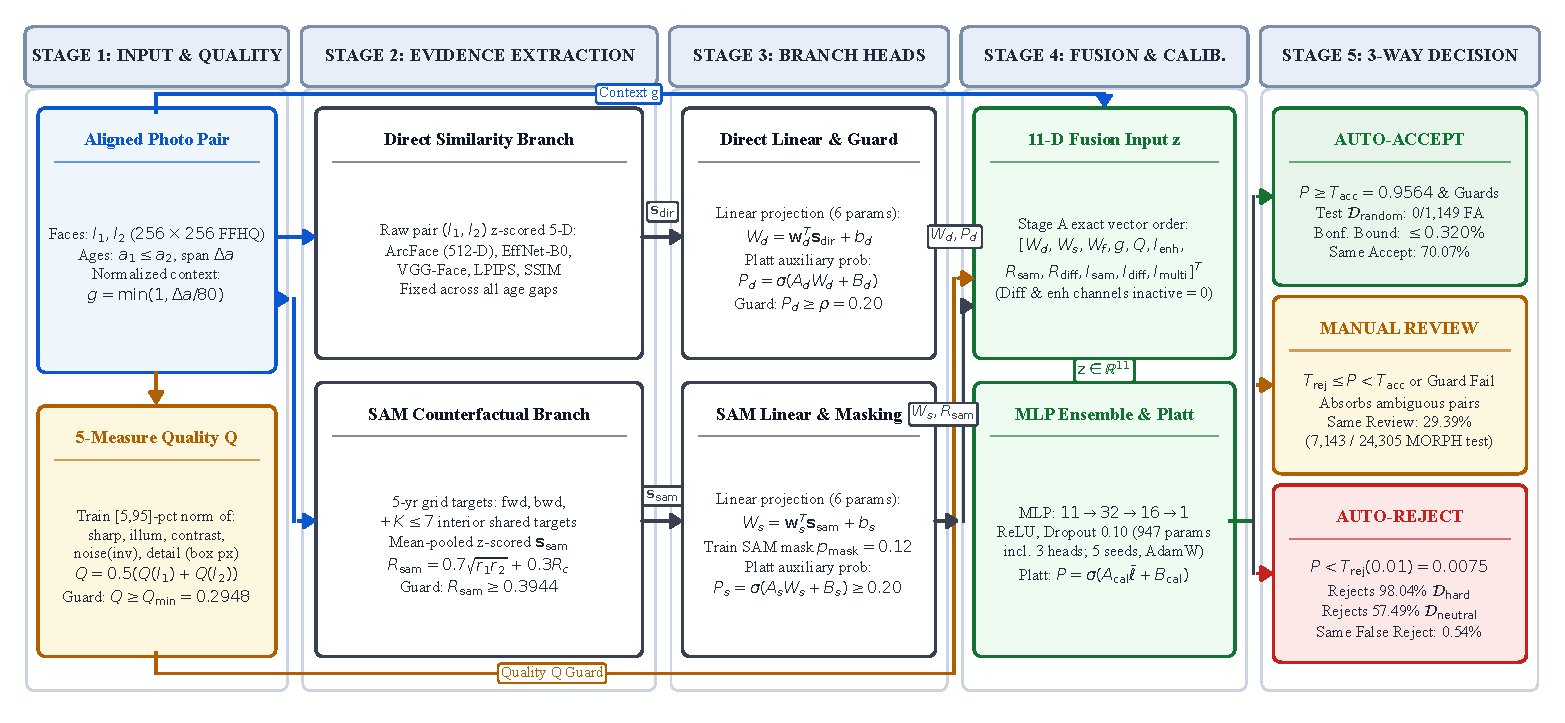
\includegraphics[width=\textwidth]{figures/fig2_architecture.pdf}
\caption{Five-stage Stage~A architecture of \sys\ matching the frozen implementation: (1)~$256\times 256$ FFHQ face alignment and 5-measure quality assessment ($Q$); (2)~direct 5-D perceptual scoring and 5-year grid SAM counterfactual progression with reliability~$R_{\text{sam}}$; (3)~branch linear learners and stochastic SAM masking ($p_{\text{mask}}=0.12$); (4)~11-D vector assembly feeding a 947-parameter 5-seed MLP ensemble and Platt calibration; and (5)~guarded three-way decision boundaries with verified MORPH Look~2 outcomes.}
\label{fig:architecture}
\end{figure*}

\subsection{Stage 1: Alignment and Five-Measure Image Quality}
\label{sec:stage1}
Images are aligned to $256\times 256$ RGB crops using FFHQ landmark geometry. For each crop~$I$, five raw perceptual quality metrics are extracted (\texttt{quality.py}): Laplacian variance sharpness (\texttt{sharp}), luminance balance $1 - |\bar{g}-128|/128$ (\texttt{illum}), grayscale standard deviation (\texttt{contrast}), inverted Immerk{\ae}r noise estimate (\texttt{noise}), and detected bounding-box pixel side (\texttt{detail}). Each measure $q_m(I)$ is min-max scaled into $[0, 1]$ using the 5th and 95th percentiles estimated exclusively on \texttt{train\_fit}:
\begin{equation}
Q(I) = \frac{1}{5} \sum_{m=1}^5 \tilde{q}_m(I), \qquad Q = \frac{1}{2}\big(Q(I_1) + Q(I_2)\big).
\end{equation}
Thus, pair quality $Q \in [0, 1]$ represents the arithmetic mean of both images' five-component quality indices. Age estimates used inside generative reliability scoring are computed via a frozen DEX estimator alongside ArcFace (\texttt{buffalo\_l}) embeddings resized to $112\times 112$.

\subsection{Stage 2: Dual-Evidence Branches and Reliability Scoring}
\label{sec:stage2}
For any aligned image pair $(A, B)$, \sys\ computes a heterogeneous five-score vector $\vect{s}_{\text{raw}}(A, B) \in \mathbb{R}^5$:
\begin{equation}
\vect{s}_{\text{raw}}(A, B) = \big[ s_{\text{arc}},\, s_{\text{eff}},\, s_{\text{vgg}},\, d_{\text{lpips}},\, s_{\text{ssim}} \big]^T,
\end{equation}
where $s_{\text{arc}}, s_{\text{eff}}, s_{\text{vgg}}$ denote cosine similarities of 512-D ArcFace~\cite{deng2019arcface}, EfficientNet-B0~\cite{tan2019efficientnet}, and VGG-Face~\cite{parkhi2015vgg} descriptors, $d_{\text{lpips}}$ is AlexNet LPIPS distance~\cite{zhang2018lpips}, and $s_{\text{ssim}}$ is structural similarity~\cite{wang2004ssim}.

\subsubsection{Direct Branch}
Direct comparison scores are z-standardized using \texttt{train\_fit} means and standard deviations $(\boldsymbol{\mu}_d, \boldsymbol{\sigma}_d)$:
\begin{equation}
\vect{s}_{\text{dir}} = \big(\vect{s}_{\text{raw}}(I_1, I_2) - \boldsymbol{\mu}_d\big) \oslash \boldsymbol{\sigma}_d.
\end{equation}

\subsubsection{SAM Counterfactual Branch}
Given chronological ages $a_1 \le a_2$, target ages are snapped to a canonical 5-year progression grid (ties rounded upward, \texttt{gap.py}): forward target $t_{\text{fwd}} = \text{snap}(a_2)$, backward target $t_{\text{bwd}} = \text{snap}(a_1)$, and interior shared targets $\{t_k\}_{k=1}^{K} \subset (a_1, a_2)$ uniformly subsampled to at most $K_{\max} = 7$ grid points. Using frozen SAM~\cite{alaluf2021sam} syntheses $(\hat{I}_1^{(t)}, \hat{I}_2^{(t)})$, each comparison vector $\vect{s}_{\text{raw}}$ is standardized via \texttt{train\_fit} SAM branch statistics $(\boldsymbol{\mu}_s, \boldsymbol{\sigma}_s)$ into $\vect{z}_{\text{fwd}}$, $\vect{z}_{\text{bwd}}$, and $\{\vect{z}_{\text{sh},k}\}_{k=1}^{K_{\text{used}}}$. Missing generations are masked rather than imputed. Letting $\vect{b} = \frac{1}{2}(\vect{z}_{\text{fwd}} + \vect{z}_{\text{bwd}})$, when bidirectional synthesis succeeds ($I_{\text{sam}} = 1$), the SAM score vector averages bidirectional and shared evidence:
\begin{equation}
\vect{s}_{\text{sam}} =
\begin{cases}
\frac{1}{2}\vect{b} + \frac{1}{2}\Big(\frac{1}{K_{\text{used}}}\sum_{k=1}^{K_{\text{used}}} \vect{z}_{\text{sh},k}\Big), & K_{\text{used}} \ge 1, \\
\vect{b}, & K_{\text{used}} = 0.
\end{cases}
\end{equation}

\subsubsection{Synthesis Reliability \texorpdfstring{$R_{\text{sam}}$}{R\_sam}}
Each generated image $\hat{I}$ receives a per-target reliability score $r_{\text{tgt}} \in [0, 1]$ averaging three equally weighted terms (\texttt{pairvec.py}): identity preservation relative to its source ($\max(0, \cos(f_{\text{arc}}(\hat{I}), f_{\text{arc}}(I)))$), bias-adjusted age accuracy $R_a = 1 - \min(1, \max(0, |\hat{a} - \bar{e}_{\text{age}} - t| - \epsilon_{\text{age}}) / (2\epsilon_{\text{age}}))$, and generated-crop quality $Q(\hat{I})$. Averaging $r_{\text{tgt}}$ across all available syntheses for faces 1 and 2 gives $(r_1, r_2)$, combined with inter-target ArcFace cosine spread $s_{\text{spread}}$ normalized by the \texttt{train\_fit} 95th percentile $\sigma_{\max}$:
\begin{multline}
R_{\text{sam}} = 0.7 \sqrt{\max(r_1, 0)\max(r_2, 0)} \\
+ 0.3\big(1 - \min(1, s_{\text{spread}} / \sigma_{\max})\big),
\end{multline}
setting $R_{\text{sam}} = 0$ if bidirectional SAM generation is unavailable.

\subsection{Stage 3--4: Linear Heads, Fusion MLP, Training, and Calibration}
Each branch score vector passes through a 6-parameter linear head ($\vect{w}_b^T \vect{s}_b + b_b$):
\begin{equation}
W_d = \vect{w}_d^T \vect{s}_{\text{dir}} + b_d, \qquad W_s = \vect{w}_s^T \vect{s}_{\text{sam}} + b_s,
\end{equation}
plus an inactive Stage~A third head $W_f$ (receiving zero inputs, reducing to a learned scalar bias) retained for extensibility. Separate Platt scalers~\cite{platt1999} fitted on \texttt{train\_val} convert logits to branch guardrail probabilities: $P_d = \sigma(A_d W_d + B_d)$ and $P_s = \sigma(A_s W_s + B_s)$.

Consistent with \texttt{fusion.py}, the 11-dimensional fusion vector concatenates branch scalars and eight context variables in exact index order:
\begin{equation}
\vect{z} = \big[ W_d, W_s, W_f, g, Q, I_{\text{enh}}, R_{\text{sam}}, R_{\text{diff}}, I_{\text{sam}}, I_{\text{diff}}, I_{\text{multi}} \big]^T,
\end{equation}
where Stage~A fixes inactive enhancement and diffusion slots ($I_{\text{enh}} = R_{\text{diff}} = I_{\text{diff}} = 0$), $I_{\text{sam}} \in \{0, 1\}$, and $I_{\text{multi}} = \mathbb{I}(K_{\text{used}} \ge 1)$. A compact MLP ($11 \!\to\! 32 \!\to\! 16 \!\to\! 1$, ReLU activations, dropout $0.10$) processes $\vect{z}$; including all three linear heads, each seed model comprises exactly $18 + 929 = 947$ trainable weights.

\textbf{Training \& Deep Learning Protocol:} Five ensemble seeds are trained strictly on \texttt{train\_fit} using AdamW (selected via \texttt{train\_val} grid search over $\text{lr} \in \{10^{-3}, 3\times 10^{-3}\}$ and $\text{wd} \in \{10^{-4}, 10^{-2}\}$, selecting $\text{lr}=3\times 10^{-3}, \text{wd}=10^{-2}$), mini-batch size $2{,}048$, max $100$ epochs, and early stopping on unweighted \texttt{train\_val} log loss ($\text{patience} = 10$, $\Delta < 10^{-5}$; stopping at epochs 30, 36, 45, 47, and 27). Training pairs receive inverse gap-bin frequency weights normalized to unit mean so rare wide-gap pairs are not overwhelmed by G1 pairs. During training, each batch applies stochastic SAM branch masking with $p_{\text{mask}} = 0.12$ (zeroing $\vect{s}_{\text{sam}}, R_{\text{sam}}, I_{\text{sam}}, I_{\text{multi}}$) to prevent over-reliance on synthetic images~\cite{poh2009quality}. Mean ensemble logits $\bar{\ell}$ are calibrated on \texttt{train\_val} via Platt scaling $P = \sigma(A_{\text{cal}}\bar{\ell} + B_{\text{cal}})$ and verified for prior-matching bin calibration error in \texttt{reliability\_by\_bin.csv} (maximum absolute bin deviation $0.0011$ across G1--G3).

\subsection{Stage 5: Guards, Threshold Freezing, and Cryptographic Sealing}
To prevent outlier extrapolation (\texttt{thresholds.py}, \texttt{p78\_calibrate\_freeze.py}), auto-acceptance requires the composite guard predicate:
\begin{equation}
\mathcal{G}(\vect{z}) =
\begin{cases}
\mathbb{I}(Q \ge Q_{\min}) \cdot \mathbb{I}(P_d \ge \rho), & I_{\text{sam}} = 0, \\
\begin{aligned}[t]
&\mathbb{I}(Q \ge Q_{\min}) \cdot \mathbb{I}(P_d \ge \rho) \\
&\quad \cdot \mathbb{I}(P_s \ge \rho) \cdot \mathbb{I}(R_{\text{sam}} \ge R_{\min}),
\end{aligned} & I_{\text{sam}} = 1,
\end{cases}
\end{equation}
where $Q_{\min} = 0.2948$ and $R_{\min} = 0.3944$ are the empirical 5th percentiles measured on \texttt{train\_fit} (\texttt{thresholds.json}), and $\rho \in \{0.20, 0.35, 0.50\}$ is chosen during calibration ($\rho = 0.20$ for \sys\ Full).

On the sequestered calibration partition, let $P_{(1)} \ge P_{(2)} \ge \dots$ denote sorted calibrated probabilities of guard-passing different-person pairs. Thresholds are computed as:
\begin{align}
T_{\text{acc}} &= P_{(1)} + \max\Big(0.001,\; \frac{1}{2}\big(P_{(1)} - P_{(5)}\big)\Big), \\
T_{\text{rej}}(\beta) &= \text{Quantile}_{\beta}\big(\{P_i : i \in \mathcal{D}_{\text{same}}^{\text{cal}}\}\big).
\end{align}
All model checkpoints, standardizers, and thresholds are saved, SHA-256 hashed, and frozen prior to accessing test.

\section{Experimental Setup and Protocols}
\label{sec:setup}

\subsection{Datasets, Quarantine Hygiene, and Splits}
\textbf{MORPH Album 2~\cite{ricanek2006morph}:} Automated identity-clustering hygiene prior to partitioning detected 858 inconsistent or merged identities (6.4\% of dataset identities), which were permanently quarantined. Remaining clean identities were partitioned person-disjointly into Training (\texttt{train\_fit} + \texttt{train\_val}, 60\%), Calibration (20\%, $338{,}871$ evaluation pairs), and Test (20\%, $339{,}011$ primary evaluation pairs: $24{,}305$ genuine same, $1{,}149$ \texttt{D\_random}, $277{,}822$ \texttt{D\_all\_random}, and $35{,}735$ \texttt{D\_hard}), plus $2{,}790$ neutral hard impostors.

\textbf{FG-NET~\cite{lanitis2002fgnet}:} To measure zero-retraining cross-dataset generalization across uncontrolled photos (ages 0--69), we evaluate MORPH-frozen models on 5,797 genuine and 20,000 random impostor pairs (All Ages), as well as the adult subset ($a_1, a_2 \ge 16$; 1,456 genuine and 3,670 impostor pairs). As recorded transparently in Limitations (Section~\ref{sec:limitations}), the $\ge 16$ adult threshold was identified post hoc after inspecting pediatric false accepts on All Ages.

\subsection{Evaluation Pools and Baselines}
To avoid circular ArcFace mining bias, test evaluation includes: (1) $\mathcal{D}_{\text{random}}$ ($N=1{,}149$ bipartite same-sex disjoint pairs); (2) $\mathcal{D}_{\text{all\_random}}$ ($N=277{,}822$ pairs sampled with replacement); (3) $\mathcal{D}_{\text{hard}}$ ($N=35{,}735$ same-sex top-5 ArcFace impostors); and (4) $\mathcal{D}_{\text{neutral}}$ ($N=2{,}790$ \texttt{D\_by\_both} overlap/combined top-1\% hard impostors mined independently by Siamese CNN and ViT without ArcFace or SAM).

We compare \sys\ against direct baselines (\texttt{ArcFace Only}, \texttt{ArcFace No Guards}, \texttt{Direct 5-Score LogReg}, \texttt{Direct-Only MLP}, \texttt{No Shared Targets}) and three end-to-end learned comparators calibrated under the identical zero-calibration-FA threshold rule:
\begin{itemize}
    \item \textbf{Siamese CNN~\cite{chopra2005siamese}:} ImageNet-pretrained ResNet-18 backbone on $128\times 128$ crops with concatenation head $[|e_1-e_2|, e_1 \odot e_2]$, trained with AdamW ($\text{lr}=3\times 10^{-4}$ backbone / $1.5\times 10^{-3}$ head, 6 max epochs, stopped epoch 4 at \texttt{val\_logloss} $=0.1950$).
    \item \textbf{Siamese ViT~\cite{dosovitskiy2021vit}:} ImageNet-21k pretrained ViT-Base-16 ($224\times 224$, $\text{lr}=2\times 10^{-5}$, 3 epochs; noted as an unconverged training cap where \texttt{val\_logloss} dropped $0.1847 \!\to\! 0.1593 \!\to\! 0.1285$).
    \item \textbf{VLM (Qwen2-VL-2B)~\cite{wang2024qwen2vl,hu2022lora}:} 4-bit LoRA ($r=16, \alpha=16$) fine-tuned for 1 epoch on 8,000 balanced pairs (\texttt{Yes}/\texttt{No} logit difference), scored strictly on the $5{,}670$-pair calibration common subset and FG-NET (absent from MORPH test).
\end{itemize}
All 95\% confidence intervals in test and FG-NET tables are computed via 500 subject-clustered bootstrap resamples~\cite{bolle2004subsets,schuckers2010book}.

\section{Results, Reconciliation, and Sensitivity}
\label{sec:results}

\begin{table*}[t]
\centering
\caption{Primary Evaluation on Person-Disjoint MORPH Test Split at $\beta = 1.0\%$ ($N_{\text{same}} = 24{,}305$, $N_{\text{random}} = 1{,}149$, $N_{\text{all\_random}} = 277{,}822$, $N_{\text{hard}} = 35{,}735$, $N_{\text{neutral}} = 2{,}790$). Source: \texttt{extended\_test.csv} (Look 2).}
\label{tab:main_results}
\footnotesize
\setlength{\tabcolsep}{4.5pt}
\begin{tabular}{@{}lcccccc@{}}
\toprule
\textbf{Method} & \makecell{\textbf{Same Accept}\\\textbf{(\%)}} & \makecell{\textbf{Random FA}\\\textbf{$\mathcal{D}_{\text{random}}$}} & \makecell{\textbf{All-Random FA}\\\textbf{$\mathcal{D}_{\text{all\_random}}$}} & \makecell{\textbf{Hard FA}\\\textbf{$\mathcal{D}_{\text{hard}}$}} & \makecell{\textbf{Hard Reject}\\\textbf{$\mathcal{D}_{\text{hard}}$ (\%)}} & \makecell{\textbf{Neutral Reject}\\\textbf{$\mathcal{D}_{\text{neutral}}$ (\%)}} \\
\midrule
\textbf{\sys\ (Full)} & 70.07 & 0 & 0 & 5 & \textbf{98.04} & \textbf{57.49} \\
\sys\ (No Shared Targets) & 83.91 & 0 & 0 & 0 & 97.85 & 53.98 \\
ArcFace Only (Guarded) & 89.45 & 0 & 0 & 0 & 0.00 & 28.46 \\
ArcFace (No Guards) & \textbf{93.58} & 0 & 0 & 0 & 0.00 & 28.46 \\
Direct 5-Score LogReg & 87.10 & 0 & 0 & 0 & 0.00 & 22.40 \\
Direct-Only MLP & 0.00 & 0 & 0 & 0 & 97.77 & 49.96 \\
Siamese CNN (ResNet-18) & 0.21 & 0 & 0 & 0 & 9.86 & n/a$^\dagger$ \\
Siamese ViT (ViT-B/16) & 0.00 & 0 & 0 & 0 & 10.04 & n/a$^\dagger$ \\
\bottomrule
\multicolumn{7}{@{}l@{}}{\footnotesize $^\dagger$Omitted from $\mathcal{D}_{\text{neutral}}$ ($D_{\text{by\_both}}$) test evaluation because Siamese CNN and ViT scores were used to mine the neutral hard-impostor set.}\\
\multicolumn{7}{@{}l@{}}{\footnotesize Note: LoRA-adapted VLM (Qwen2-VL-2B) was not evaluated on MORPH \texttt{test}; see Table~\ref{tab:cal_subset} for calibration common-subset evaluation.}
\end{tabular}
\end{table*}



\subsection{Primary MORPH Test Comparison}
Table~\ref{tab:main_results} and Fig.~\ref{fig:results}(a) summarize Look~2 MORPH test performance at $\beta = 1.0\%$. Complete 95\% subject-clustered bootstrap intervals are detailed in Appendix Table~\ref{tab:supp_intervals}. Three quantitative patterns emerge:
\begin{enumerate}
    \item \textbf{Zero Random False Accepts:} \sys\ (Full) produces zero false accepts on $\mathcal{D}_{\text{random}}$ ($0/1{,}149$) and $\mathcal{D}_{\text{all\_random}}$ ($0/277{,}822$), supporting the analytical $0.320\%$ bound on $\mathcal{D}_{\text{random}}$ across both logged looks.
    \item \textbf{Hard-Impostor Rejection vs.\ Nominal Acceptance Trade-Off:} Guarded ArcFace achieves higher same-person auto-accept ($89.45\%$ vs.\ $70.07\%$) and higher random impostor rejection ($63.53\%$ vs.\ $34.03\%$ on $\mathcal{D}_{\text{random}}$), but auto-rejects $0.00\%$ of ArcFace-mined $\mathcal{D}_{\text{hard}}$ and only $28.46\%$ of $\mathcal{D}_{\text{neutral}}$, routing all $\mathcal{D}_{\text{hard}}$ pairs to human review. \sys\ filters $98.04\%$ of $\mathcal{D}_{\text{hard}}$ ($35{,}034/35{,}735$, with $5$ residual false accepts) and $57.49\%$ of unbiased $\mathcal{D}_{\text{neutral}}$ ($1{,}604/2{,}790$).
    \item \textbf{Minimax Threshold Collapse of Learned Comparators:} Under the identical zero-calibration-FA rule, Siamese CNN ($0.21\%$) and Siamese ViT ($0.00\%$) collapse to near-zero genuine throughput because heavy impostor tails drive $T_{\text{acc}}$ to $0.982$ and $1.001$, respectively.
\end{enumerate}

\begin{figure*}[t]
\centering
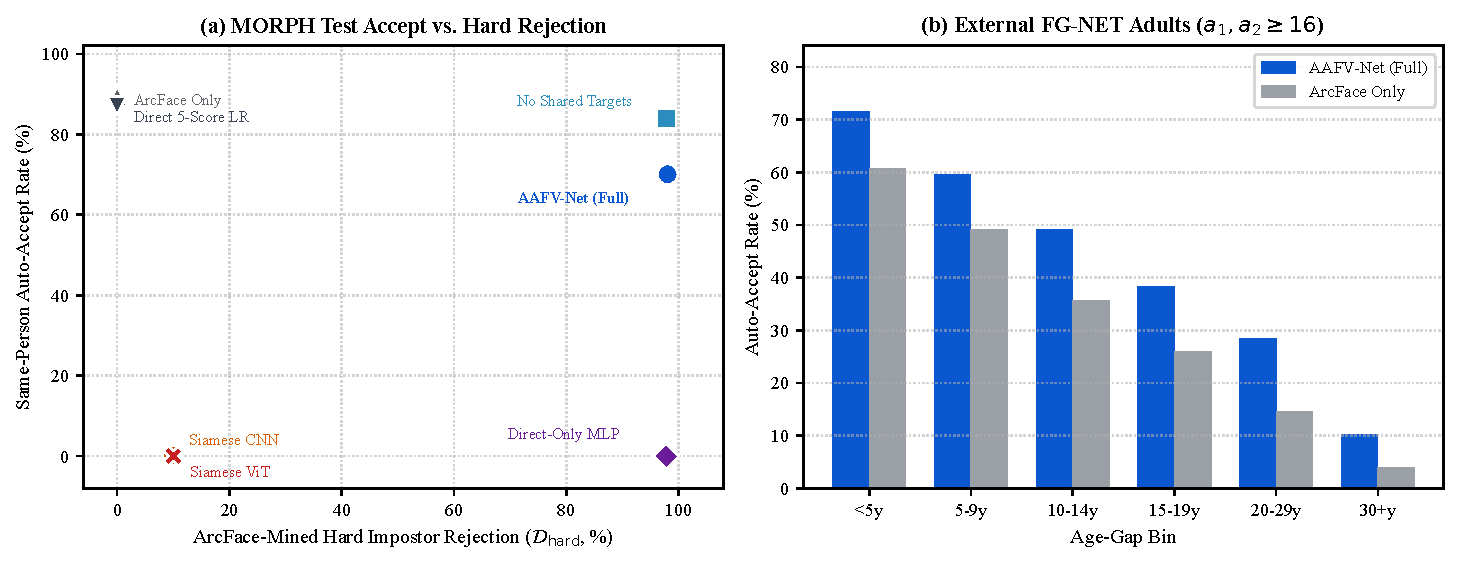
\includegraphics[width=0.95\textwidth]{figures/fig3_results.pdf}
\caption{Primary empirical findings. (a)~MORPH \texttt{test} same-person auto-accept versus ArcFace-mined hard impostor rejection at $\beta=1.0\%$, contrasting high-throughput single-branch matchers (zero hard rejection), collapsed end-to-end learners, and \sys. (b)~Zero-shot transfer on FG-NET adults ($a_1, a_2 \ge 16$) across all six age-gap bins, where \sys\ improves genuine acceptance in every stratum.}
\label{fig:results}
\end{figure*}

\subsection{Calibration Subset Discrimination and VLM Assessment}
Because Qwen2-VL-2B was scored solely on calibration common subsets, Table~\ref{tab:cal_subset} and Fig.~\ref{fig:outcomes} isolate calibration-split discrimination and outcome shares across all comparators including VLM. Despite achieving competitive unthresholded AUC on calibration $\mathcal{D}_{\text{hard}}$ ($0.972$ for ViT, $0.953$ for CNN, $0.906$ for VLM), all three fail to reach usable zero-FA auto-accept ($0.00\%$--$0.27\%$) and reject only $10.20\%$--$12.20\%$ of hard impostors, whereas \sys\ attains $\text{AUC}=0.998$ and $\text{TPR}=0.973$ at $\text{FPR}=10^{-3}$.

\begin{table*}[t]
\centering
\caption{Calibration Split Discrimination and Three-Way Decision Comparison ($\beta = 1.0\%$). Ranking metrics are computed on full calibration $\mathcal{D}_{\text{hard}}$ ($N=35{,}769$) except VLM ($N=1{,}500$). Decision rates come from the label-free calibration common subset ($N_{\text{same}}=1{,}500$, $N_{\text{random}}=1{,}170$, $N_{\text{hard}}=1{,}500$; \texttt{decision\_table\_calibration.csv}).}
\label{tab:cal_subset}
\footnotesize
\setlength{\tabcolsep}{4.5pt}
\begin{tabular}{@{}lccccccc@{}}
\toprule
\textbf{Architecture} & \makecell{\textbf{Cal. AUC}\\\textbf{($\mathcal{D}_{\text{hard}}$)}} & \makecell{\textbf{TPR @}\\\textbf{$\text{FPR}=10^{-3}$}} & \makecell{\textbf{Frozen}\\\textbf{$T_{\text{acc}}$}} & \makecell{\textbf{Same Accept}\\\textbf{(\%)}} & \makecell{\textbf{Random Rej.}\\\textbf{(\%)}} & \makecell{\textbf{Hard Rej.}\\\textbf{(\%)}} & \makecell{\textbf{Eval. Pool}\\\textbf{($N_{\text{hard}}$ AUC)}} \\
\midrule
\textbf{\sys\ (Full)} & \textbf{0.998} & \textbf{0.973} & 0.956 & 74.13 & 26.15 & \textbf{98.20} & Full Cal. (35,769) \\
ArcFace Only (Guarded) & 0.980 & 0.969 & 0.850 & \textbf{87.20} & 47.95 & 0.00 & Full Cal. (35,769) \\
Direct 5-Score LogReg & 0.981 & 0.971 & 0.913 & 84.27 & \textbf{57.26} & 0.00 & Full Cal. (35,769) \\
Direct-Only MLP & 0.998 & 0.971 & 1.042 & 0.00 & 26.67 & 98.47 & Full Cal. (35,769) \\
Siamese CNN (ResNet-18) & 0.953 & 0.311 & 0.982 & 0.27 & 49.74 & 10.87 & Full Cal. (35,769) \\
Siamese ViT (ViT-B/16) & 0.972 & 0.605 & 1.001 & 0.00 & 51.97 & 12.20 & Full Cal. (35,769) \\
VLM (Qwen2-VL-2B LoRA) & 0.906 & 0.054 & 0.998 & 0.00 & 47.01 & 10.20 & Common Subset (1,500) \\
\bottomrule
\end{tabular}
\end{table*}



\begin{figure*}[t]
\centering
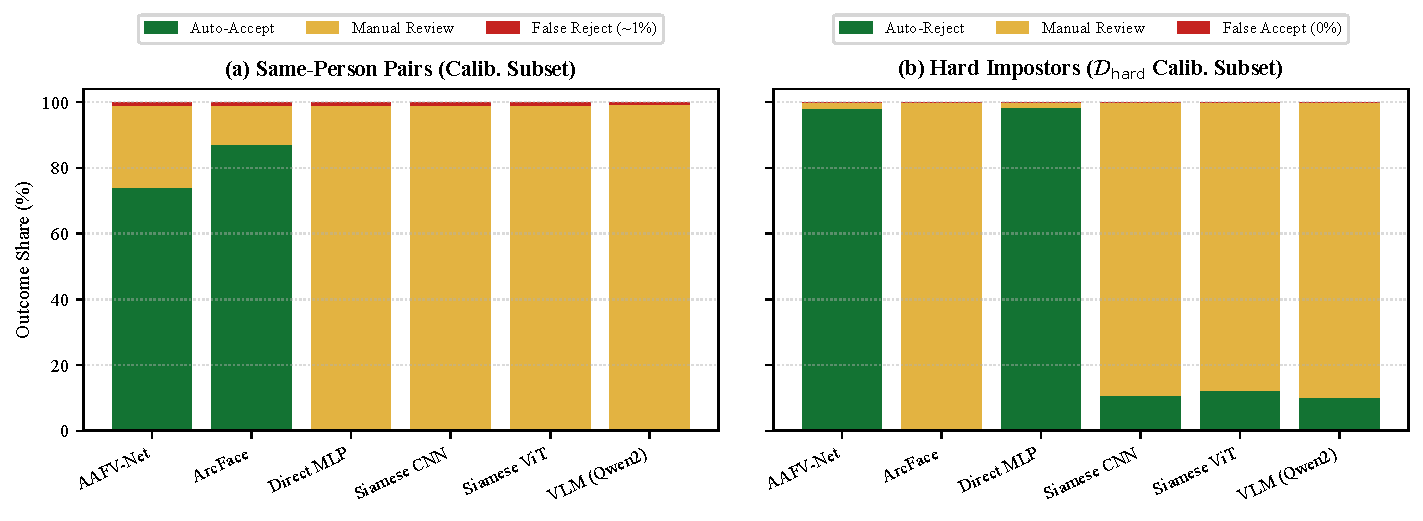
\includegraphics[width=0.94\textwidth]{figures/fig7_decision_outcomes.pdf}
\caption{Decision outcome partitioning on the calibration common subset ($\beta = 1.0\%$, $N_{\text{same}}=1{,}500$, $N_{\text{hard}}=1{,}500$, zero calibration FAs). (a)~Same-person outcomes illustrating near-complete manual-review fallback for Direct MLP, Siamese CNN/ViT, and Qwen2-VL-2B. (b)~Hard-impostor ($\mathcal{D}_{\text{hard}}$) outcomes showing $98.20\%$ auto-rejection by \sys\ versus $0.00\%$ for ArcFace and $10.20\%$--$12.20\%$ for deep comparators.}
\label{fig:outcomes}
\end{figure*}

\subsection{Reconciliation of Test Look 1 and Test Look 2}
Table~\ref{tab:reconciliation} reconciles both logged test accesses recorded in \texttt{test\_access.log}. Look~1 evaluated Stage~A \texttt{thresholds.json} prior to quantile calibration (\texttt{T\_reject} $= -0.000385$), yielding $79.74\%$ genuine accept ($0\%$ auto-reject) and $3$ hard FAs. Look~2 calibrated \texttt{T\_reject} $= 0.007541$ at $\beta = 1.0\%$ on \texttt{frozen.pkl} (SHA-256 \texttt{a47c916b...35b9}), activating $98.04\%$ hard-impostor filtering while adjusting genuine accept to $70.07\%$ ($29.39\%$ review, $0.54\%$ same-person false reject) and observing $5$ hard FAs. Both looks recorded zero false accepts on $\mathcal{D}_{\text{random}}$ and $\mathcal{D}_{\text{all\_random}}$.

\begin{table}[t]
\centering
\caption{Audit Reconciliation Between Test Look 1 and Test Look 2 on Protected MORPH \texttt{test} Split.}
\label{tab:reconciliation}
\footnotesize
\setlength{\tabcolsep}{3.5pt}
\resizebox{\columnwidth}{!}{%
\begin{tabular}{@{}lcc@{}}
\toprule
\textbf{Protocol Item / Metric} & \textbf{Look 1 (Initial)} & \textbf{Look 2 (Extended)} \\
\midrule
Evaluation Script & \texttt{p9\_test.py} & \texttt{p12\_extended.py} \\
Logged UTC Timestamp & 2026-11-05 21:42:09 & 2026-11-07 19:45:00 \\
Frozen Artifact & \texttt{thresholds.json} & \texttt{frozen.pkl} \\
SHA-256 Prefix\ldots Suffix & \texttt{4b7af977\ldots 2cfe}$^\dagger$ & \texttt{a47c916b\ldots 35b9} \\
Accept Threshold $T_{\text{acc}}$ & 0.956575 & 0.956438 \\
Reject Threshold $T_{\text{rej}}$ & $-0.000385$ & 0.007541 \\
Target False-Reject Budget $\beta$ & Uncalibrated & Calibrated ($1.0\%$) \\
\midrule
Same-Person Auto-Accept & 79.74\% (19,382/24,305) & 70.07\% (17,030/24,305) \\
Same-Person Manual Review & 20.26\% (4,923/24,305) & 29.39\% (7,143/24,305) \\
Same-Person Auto-Reject & 0.00\% (0/24,305) & 0.54\% (132/24,305) \\
$\mathcal{D}_{\text{random}}$ False Accepts & 0 / 1,149 & 0 / 1,149 \\
$\mathcal{D}_{\text{all\_random}}$ False Accepts & 0 / 277,822 & 0 / 277,822 \\
$\mathcal{D}_{\text{hard}}$ False Accepts & 3 / 35,735 (0.008\%) & 5 / 35,735 (0.014\%) \\
$\mathcal{D}_{\text{hard}}$ Auto-Reject & 0.00\% (0/35,735) & 98.04\% (35,034/35,735) \\
\bottomrule
\multicolumn{3}{@{}l@{}}{\footnotesize $^\dagger$LF-normalized digest logged by \texttt{test\_access.log} (\texttt{8c2fdd00\ldots e147} with CRLF).}
\end{tabular}%
}
\end{table}


\subsection{Sensitivity Across False-Reject Budget \texorpdfstring{$\beta$}{beta}}
Fig.~\ref{fig:beta_sweep} tracks MORPH test impostor rejection across $\beta \in \{0.005, 0.010, 0.020\}$ (\texttt{extended\_test.csv}). Because $\beta$ governs only $T_{\text{rej}}(\beta)$, same-person accept rates remain fixed ($70.07\%$) while \sys\ increases $\mathcal{D}_{\text{hard}}$ rejection from $96.33\%$ to $98.75\%$ and $\mathcal{D}_{\text{neutral}}$ rejection from $30.00\%$ to $92.58\%$. Guarded ArcFace rejects $0.00\%$ of $\mathcal{D}_{\text{hard}}$ at $\beta \le 0.010$ and reaches $71.94\%$ only when $\beta$ is relaxed to $0.020$.

\begin{figure}[t]
\centering
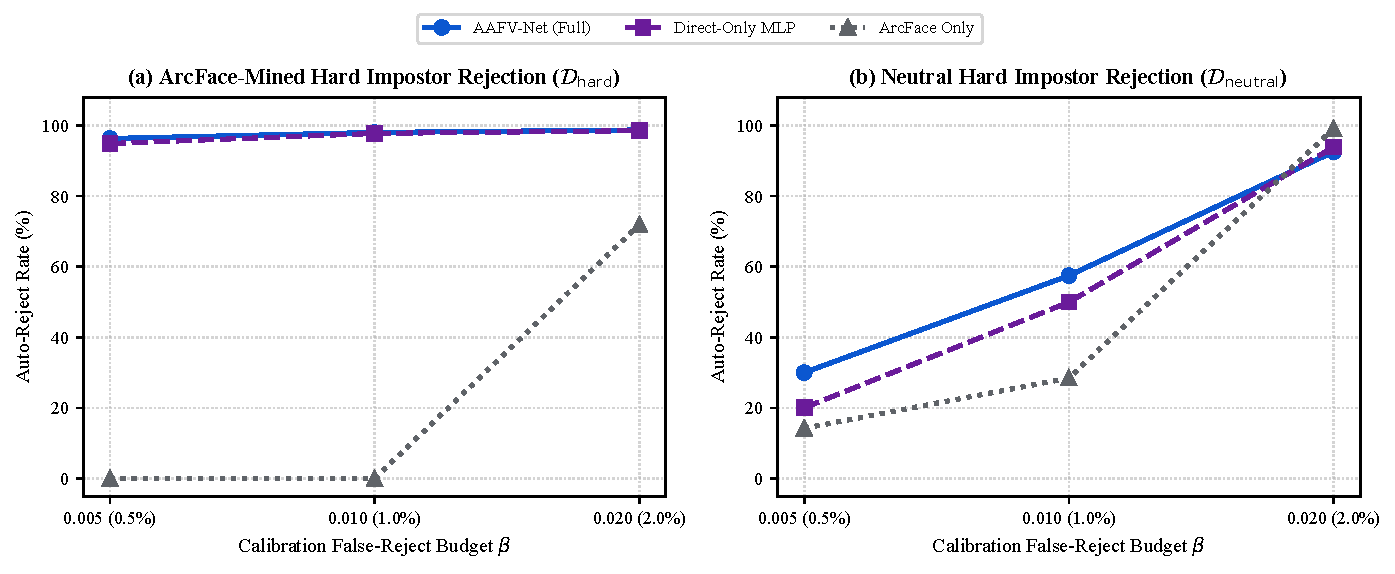
\includegraphics[width=\columnwidth]{figures/fig6_beta_sweep.pdf}
\caption{MORPH \texttt{test} auto-rejection sensitivity across calibration false-reject budget $\beta \in \{0.005, 0.010, 0.020\}$ (\texttt{extended\_test.csv}).}
\label{fig:beta_sweep}
\end{figure}

\section{Longitudinal Generalization and Ablations}
\label{sec:generalization}

\subsection{Age-Gap Behavior on MORPH vs.\ FG-NET Transfer}
Table~\ref{tab:gap_analysis} and Fig.~\ref{fig:gap_neutral}(a) report MORPH test genuine auto-accept across the six verified code bins (G1: 0--4y through G6: 30+y). Both \sys\ and ArcFace decline sharply across G4--G5 ($15$--$29$ years, sparse mugshot strata with $N=75$ and $137$), and ArcFace exceeds \sys\ on every MORPH bin because ArcFace is unconstrained by hard-impostor rejection.

Conversely, Table~\ref{tab:fgnet} and Fig.~\ref{fig:results}(b) show that under larger cross-domain longitudinal shifts on external FG-NET portraits, \sys\ surpasses ArcFace across all six age-gap bins: overall adult auto-accept rises from $40.38\%$ to $51.92\%$ ($+28.6\%$ relative) with zero impostor FAs ($0/3{,}670$), reaching $28.49\%$ vs.\ $14.52\%$ at $20$--$29$ years and $10.26\%$ vs.\ $3.85\%$ at $30+$ years. Crucially, we preserve two negative FG-NET results: (1) adult impostor rejection is lower than ArcFace ($55.04\%$ vs.\ $71.28\%$); and (2) on All Ages, \sys\ incurred $4/20{,}000$ impostor FAs exclusively involving young children aged $0$--$4$ years (identified in upstream \texttt{p12\_inspect\_fa.py} audits as pairs \texttt{069A00/023A00}, \texttt{019A00/024A00}, \texttt{021A03/064A04}, and \texttt{070A00/010A01}), confirming StyleGAN aging instability under rapid pediatric growth and restricting safe operational scope to adults ($a \ge 16$).

\begin{table}[t]
\centering
\caption{MORPH Test Same-Person Auto-Accept Rate (\%) Stratified by Verified Code Age-Gap Bins (\texttt{gap.py}, \texttt{extended\_test.csv}).}
\label{tab:gap_analysis}
\footnotesize
\setlength{\tabcolsep}{3.0pt}
\begin{tabular}{@{}lcccccc@{}}
\toprule
\textbf{Method} & \makecell{\textbf{G1}\\\textbf{0--4y}\\\scriptsize(23,631)} & \makecell{\textbf{G2}\\\textbf{5--9y}\\\scriptsize(266)} & \makecell{\textbf{G3}\\\textbf{10--14y}\\\scriptsize(184)} & \makecell{\textbf{G4}\\\textbf{15--19y}\\\scriptsize(75)} & \makecell{\textbf{G5}\\\textbf{20--29y}\\\scriptsize(137)} & \makecell{\textbf{G6}\\\textbf{30+y}\\\scriptsize(12)} \\
\midrule
\sys\ (Full) & 71.03 & 56.39 & 45.65 & 1.33 & 2.19 & 50.00 \\
ArcFace Only & 90.49 & 80.08 & 69.02 & 2.67 & 2.19 & 100.00 \\
\bottomrule
\end{tabular}
\end{table}


\begin{table*}[t]
\centering
\caption{External Zero-Retraining Generalization on FG-NET Using MORPH-Frozen Thresholds ($\beta=1.0\%$). Adults ($a_1,a_2 \ge 16$): 1,456 genuine / 3,670 impostor (5,126 total pairs; cut chosen post hoc). All Ages: 5,797 genuine / 20,000 impostor (25,797 total pairs). Genuine bin counts G1--G6 are (405, 356, 261, 170, 186, 78) for Adults and (1,654, 1,589, 1,081, 615, 572, 286) for All Ages (\texttt{extended\_calibration\_fg*.csv}). Intervals are 95\% subject-clustered bootstraps.}
\label{tab:fgnet}
\footnotesize
\setlength{\tabcolsep}{3.8pt}
\begin{tabular}{@{}llccccccccc@{}}
\toprule
\textbf{Cohort} & \textbf{Method} & \makecell{\textbf{Accept}\\\textbf{(\% [95\% CI])}} & \makecell{\textbf{Impostor}\\\textbf{FA}} & \makecell{\textbf{Imp.}\\\textbf{Rej. (\%)}} & \textbf{$<$5y} & \textbf{5--9y} & \textbf{10--14y} & \textbf{15--19y} & \textbf{20--29y} & \textbf{30+y} \\
\midrule
\multirow{2}{*}{\textbf{Adults ($a\ge 16$)}} & \textbf{\sys} & \textbf{51.92} [44.47, 58.41] & 0 / 3,670 & 55.04 & \textbf{71.60} & \textbf{59.55} & \textbf{49.04} & \textbf{38.24} & \textbf{28.49} & \textbf{10.26} \\
 & ArcFace Only & 40.38 [34.53, 47.38] & 0 / 3,670 & \textbf{71.28} & 60.74 & 49.16 & 35.63 & 25.88 & 14.52 & 3.85 \\
\midrule
\multirow{2}{*}{\textbf{All Ages}} & \textbf{\sys} & 29.86 [26.69, 33.34] & 4 / 20,000$^\ddagger$ & \textbf{66.45} & 59.07 & 28.95 & 14.80 & 11.71 & 9.44 & 2.80 \\
 & ArcFace Only & 21.29 [18.40, 24.22] & \textbf{0 / 20,000} & 64.42 & 45.53 & 19.19 & 9.34 & 7.32 & 4.72 & 1.05 \\
\bottomrule
\multicolumn{11}{@{}l@{}}{\footnotesize $^\ddagger$All four impostor false accepts occurred on young children aged 0--4 years, motivating restriction to adult subjects ($a \ge 16$).}
\end{tabular}
\end{table*}


\begin{figure*}[t]
\centering
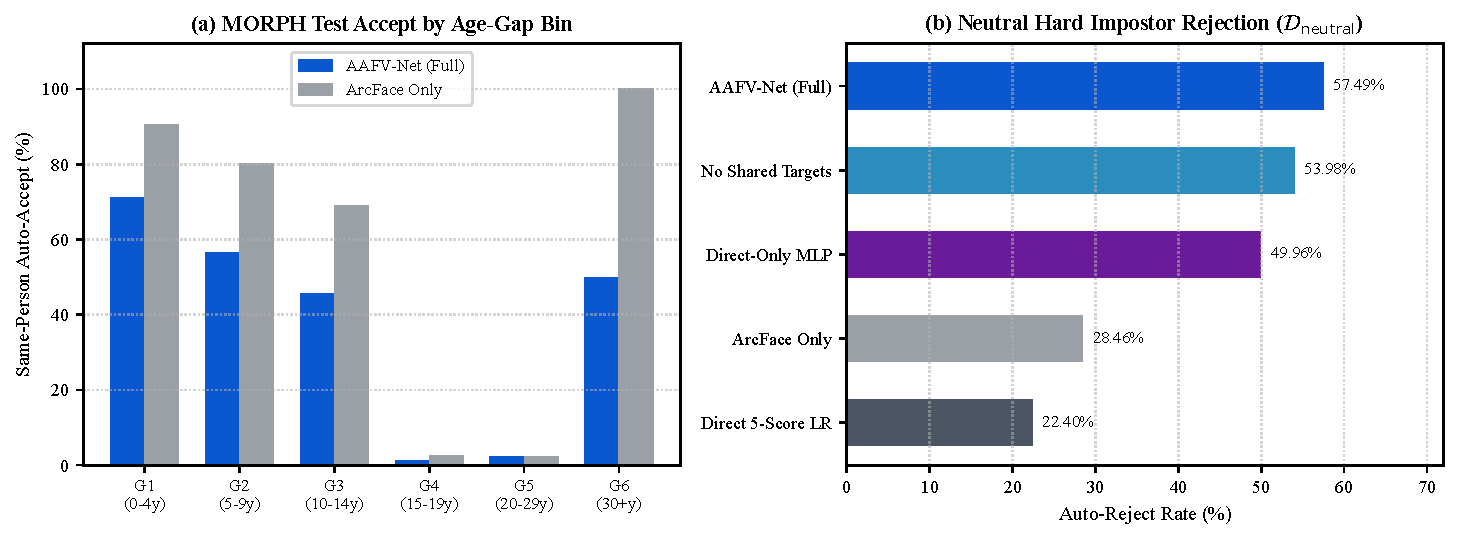
\includegraphics[width=0.95\textwidth]{figures/fig5_gap_neutral.pdf}
\caption{(a)~MORPH \texttt{test} same-person acceptance stratified across verified 6-bin age spans (\texttt{gap.py}). (b)~Rejection rates on model-neutral hard impostors ($\mathcal{D}_{\text{neutral}}, N=2{,}790$), showing shared-target counterfactuals preserve the highest unbiased hard-impostor rejection.}
\label{fig:gap_neutral}
\end{figure*}

\subsection{Component and Guard Ablations}
Table~\ref{tab:ablations} and Fig.~\ref{fig:ablations} quantify each architectural choice on the calibration common subset (\texttt{decision\_table\_calibration.csv}, $\beta=1.0\%$):
\begin{itemize}
    \item \textbf{Role of Branch Probability Guards:} Removing probability guards (\texttt{guard\_none}, \texttt{guard\_quality\_only}, \texttt{guard\_quality\_reliability}) raises $T_{\text{acc}} = 1.005 > 1$, collapsing auto-accept to $0.00\%$ identically across all three configurations. Thus, branch probability floors ($P_d, P_s \ge 0.20$) are the decisive mechanism enabling finite zero-FA acceptance thresholds.
    \item \textbf{Branch Masking and Context Inputs:} Disabling SAM masking ($p_{\text{mask}}=0$) shifts guard selection to $\rho=0.35$ and drops acceptance to $3.60\%$; removing context ($g, Q, R_{\text{sam}}$) pushes $T_{\text{acc}} = 1.042$ ($0.00\%$ accept).
    \item \textbf{Metric Parsimony vs.\ Complementarity:} Dropping ArcFace collapses accept to $0.73\%$ and hard reject to $17.87\%$, whereas dropping LPIPS reduces accept by $11.26$ pp ($74.13\% \!\to\! 62.87\%$). Conversely, dropping EfficientNet raises accept to $81.27\%$, indicating EfficientNet redundancy under calibration guards.
    \item \textbf{Shared-Targets Trade-Off:} Omitting shared grid comparisons raises accept ($74.13\% \!\to\! 84.80\%$ calibration; $83.91\%$ test with $0/35{,}735$ $\mathcal{D}_{\text{hard}}$ FAs) while lowering neutral hard rejection from $57.49\%$ to $53.98\%$ on test (Fig.~\ref{fig:gap_neutral}(b)). Following pre-registration discipline, we keep \texttt{full} as primary and report the shared-target trade-off transparently.
\end{itemize}

\begin{table}[t]
\centering
\caption{Component and Guard Ablation Study on Calibration Common Subset ($\beta = 1.0\%$, $N_{\text{same}} = 1{,}500$, $N_{\text{hard}} = 1{,}500$; \texttt{decision\_table\_calibration.csv}).}
\label{tab:ablations}
\footnotesize
\setlength{\tabcolsep}{3.5pt}
\resizebox{\columnwidth}{!}{%
\begin{tabular}{@{}lcccc@{}}
\toprule
\textbf{Ablation Variant} & \textbf{$T_{\text{acc}}$} & \textbf{Acc. (\%)} & \textbf{Rej. (\%)} & \textbf{Rand. Rej. (\%)} \\
\midrule
\textbf{Full \sys\ ($\rho=0.20$)} & 0.956 & 74.13 & \textbf{98.20} & 26.15 \\
\midrule
\textit{Metric Ablations:} & & & & \\
Drop ArcFace & 0.994 & 0.73 & 17.87 & 52.99 \\
ArcFace Score Only & 1.008 & 0.00 & 97.73 & 24.19 \\
Drop LPIPS & 1.000 & 62.87 & 97.47 & 29.32 \\
Drop SSIM & 0.989 & 72.80 & 97.40 & 23.68 \\
Drop VGG-Face & 0.976 & 73.93 & 97.20 & 19.57 \\
Drop EfficientNet & 0.978 & 81.27 & 97.60 & 20.85 \\
\midrule
\textit{Architecture \& Guard Ablations:} & & & & \\
No Branch Masking ($p=0$)$^\ast$ & 0.593 & 3.60 & 98.40 & 30.94 \\
No Context ($g,Q,R_{\text{sam}}$) & 1.042 & 0.00 & 98.07 & 24.70 \\
No Reliability ($R_{\text{sam}}$) & 0.989 & 73.27 & 97.80 & 23.85 \\
No Pair Weights & 0.985 & 74.40 & 97.33 & 24.62 \\
Forward Target Only & 0.954 & 75.07 & 98.27 & 25.98 \\
No Shared Targets & 0.997 & \textbf{84.80} & 98.27 & 29.23 \\
Shared Targets Only & 1.024 & 0.00 & 98.13 & 19.06 \\
Direct-Only MLP & 1.042 & 0.00 & 98.47 & 26.67 \\
SAM-Only MLP & 1.001 & 0.00 & 44.80 & \textbf{60.77} \\
Fusion LogReg (No MLP) & 0.869 & 64.67 & 0.00 & 57.86 \\
No Probability Guards (All 3)$^\ddagger$ & 1.005 & 0.00 & 98.20 & 26.15 \\
\bottomrule
\multicolumn{5}{@{}l@{}}{\footnotesize $^\ast$Selected $\rho = 0.35$ in calibration grid; $^\ddagger$\texttt{guard\_none}, \texttt{guard\_quality\_only},}\\
\multicolumn{5}{@{}l@{}}{\footnotesize and \texttt{guard\_quality\_reliability} produced identical rates.}
\end{tabular}%
}
\end{table}


\begin{figure}[t]
\centering
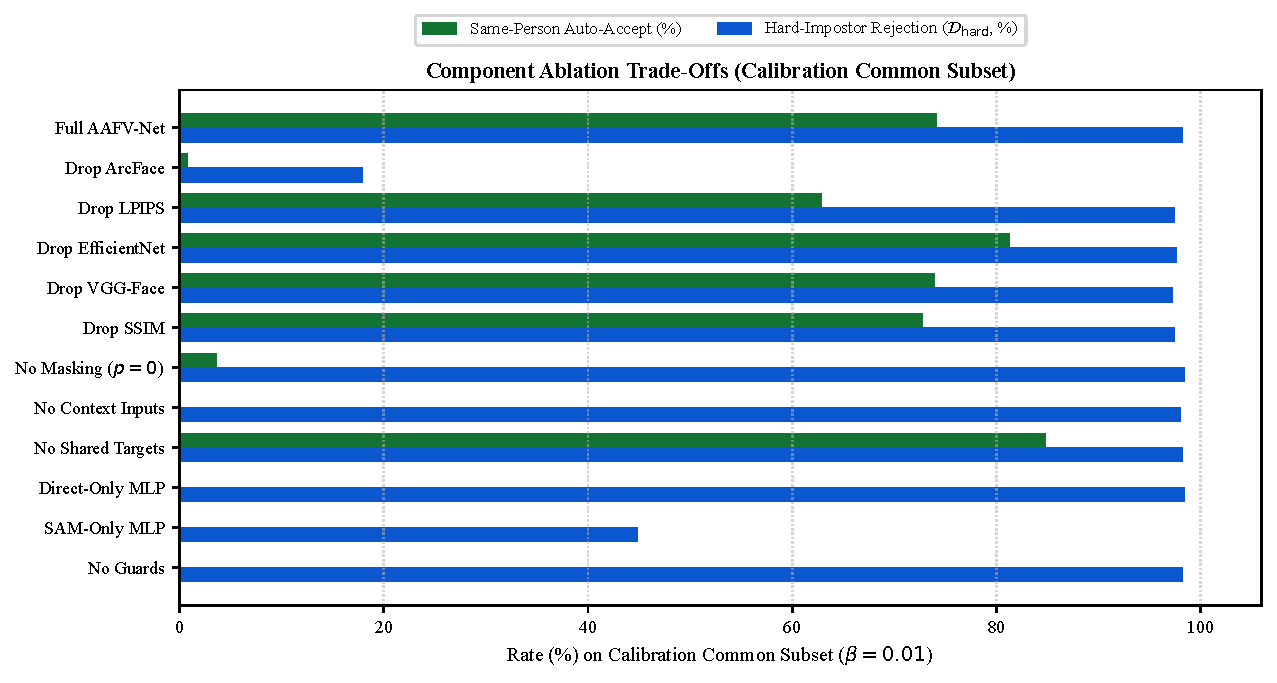
\includegraphics[width=\columnwidth]{figures/fig4_ablations.pdf}
\caption{Calibration common-subset component ablations at $\beta=1.0\%$, isolating critical collapses upon removing ArcFace, LPIPS, branch masking, context bypasses, or probability guards.}
\label{fig:ablations}
\end{figure}

\section{Fairness, Complexity, and Ethical Scope}
\label{sec:fairness}

\subsection{Demographic Parity and Residual Error Transparency}
Using the only gender-resolved test log saved on disk (\texttt{test\_pair\_zones\_look1.csv}, Look~1), Table~\ref{tab:fairness} reveals a tangible demographic acceptance gap: Male genuine pairs ($N=20{,}774$) are auto-accepted at $81.07\%$, whereas Female genuine pairs ($N=3{,}531$) are auto-accepted at $71.93\%$ ($\Delta = 9.14$ percentage points, disparate impact ratio $0.887$). Zero false accepts occurred on $\mathcal{D}_{\text{random}}$ in both sexes ($0/982$ male, $0/167$ female), while all three Look~1 hard impostor FAs occurred in the male cohort ($3/30{,}921$ vs.\ $0/4{,}814$). This female genuine-acceptance gap aligns with published TIFS biometric demographic findings~\cite{klare2012demographics,grother2019frvt_part3}. Look~2 \texttt{extended\_test.csv} did not retain per-pair sex columns, and MORPH racial subgroup metadata was not evaluated in frozen test logs; both gaps remain explicit targets for future fairness auditing. Furthermore, in contrast to visual contact sheets inspected on FG-NET false accepts, the five residual Look~2 $\mathcal{D}_{\text{hard}}$ false accepts (\texttt{5/35,735}) were not visually inspected due to test-artifact restrictions and are reported strictly numerically.

\begin{table}[t]
\centering
\caption{Sex-Disaggregated Verification Audit on Protected MORPH Test Split (Look 1 Log \texttt{test\_pair\_zones\_look1.csv}; Per-Pair Sex Metadata Was Not Saved in Look 2).}
\label{tab:fairness}
\footnotesize
\setlength{\tabcolsep}{3.5pt}
\resizebox{\columnwidth}{!}{%
\begin{tabular}{@{}lcccc@{}}
\toprule
\textbf{Cohort} & \makecell{\textbf{Same Accept}\\\textbf{(\%)}} & \makecell{\textbf{Same Review}\\\textbf{(\%)}} & \makecell{\textbf{Random FA}\\\textbf{$\mathcal{D}_{\text{random}}$}} & \makecell{\textbf{Hard FA}\\\textbf{$\mathcal{D}_{\text{hard}}$}} \\
\midrule
Male ($N_{\text{same}}=20{,}774$) & 81.07 & 18.93 & 0 / 982 & 3 / 30,921 \\
Female ($N_{\text{same}}=3{,}531$) & 71.93 & 28.07 & 0 / 167 & 0 / 4,814 \\
\midrule
Gap ($\Delta$ M$-$F / DI Ratio) & \multicolumn{2}{c}{9.14 pp (Ratio: 0.887)} & 0.00 pp & -- \\
\bottomrule
\end{tabular}%
}
\end{table}


\subsection{Parameter Decomposition and Execution Complexity}
Table~\ref{tab:complexity} decomposes verified trainable parameter counts and algorithmic execution calls without extrapolating unmeasured hardware timings for external extractors. The learned fusion stage comprises just $947$ weights per seed ($4{,}741$ parameters total across the 5-seed ensemble and Platt calibrators) and executes in $0.18\,\mu\text{s}$ per pair batched ($77.2\,\mu\text{s}$ unbatched single-pair on AMD x86-64 CPU). While the current research pipeline pre-computes SAM generations across up to $2 + 2K \le 16$ targets per pair, deployment architectures can evaluate the direct branch first and invoke SAM conditionally only for non-accepted, non-rejected pairs falling into review.

\begin{table}[t]
\centering
\caption{Exact Trainable Fusion Parameter Decomposition, Verified CPU Inference Overhead, and Pipeline Call Complexity (Excluding Unmeasured Upstream Backbone Wall-Clock Timings).}
\label{tab:complexity}
\footnotesize
\setlength{\tabcolsep}{3.5pt}
\resizebox{\columnwidth}{!}{%
\begin{tabular}{@{}lcc@{}}
\toprule
\textbf{Pipeline Stage / Component} & \textbf{Trainable Params} & \textbf{Per-Pair Execution Calls} \\
\midrule
Quality \& Landmark Alignment & 0 (analytical / pre-trained) & 2 image crops ($256\times 256$) \\
Direct Similarity Extractors & 0 (frozen backbones) & 1 direct comparison ($\vect{s}_{\text{dir}}$) \\
SAM Synthesis + Aging Metrics & 0 (frozen generators) & Up to $2 + 2K \le 16$ passes \\
Linear Heads ($W_d, W_s, W_f$) & $3 \times 6 = 18$ (12 active Stage A) & 1 linear projection/pair \\
Fusion MLP ($11\!\to\!32\!\to\!16\!\to\!1$) & $929$ (total \texttt{Fusion}: $947$) & $0.18\,\mu\text{s}$ (batched)$^\dagger$ / $77.2\,\mu\text{s}$ \\
5-Seed Ensemble + Platt Scalers & $5\times 947 + 6 = 4{,}741$ & $< 0.4\,\text{ms}$ CPU unbatched \\
\bottomrule
\multicolumn{3}{@{}l@{}}{\footnotesize $^\dagger$Measured PyTorch CPU single-seed inference on AMD x86-64 (\texttt{batch=1024} amortized vs.\ single-pair).}
\end{tabular}%
}
\end{table}


\subsection{Biometric Ethics, Privacy, and Reproducibility Disclosures}
All experiments use established secondary academic biometric benchmarks (MORPH Album~2 under academic license and FG-NET) without collecting new human subjects or releasing raw facial images. Operational scope explicitly excludes minors ($a < 16$). Upstream research dependencies (\texttt{InsightFace buffalo\_l}, \texttt{SAM}, \texttt{DEX}) carry non-commercial academic licenses requiring open-weight replacement prior to commercial deployment. No author data, results, or citations were generated or altered via generative AI tools; full code, SHA-256 manifests, and the 26-variant supplementary appendix are provided for independent verification.

\section{Discussion, Limitations, and Conclusion}
\label{sec:conclusion}

\subsection{Operational Positioning and Transparent Limitations}
\label{sec:limitations}
Collectively, Tables~\ref{tab:main_results}--\ref{tab:fairness} clarify why \sys\ complements rather than universally dominates single-branch matchers. Unconstrained ArcFace achieves higher nominal same-person accept on MORPH ($89.45\%$ vs.\ $70.07\%$) and higher random-impostor rejection, yet fails to auto-reject ArcFace-mined look-alikes ($0.00\%$ at $\beta \le 1\%$). Conversely, end-to-end Siamese CNN/ViT and Qwen2-VL comparators yield strong raw discrimination but collapse to $\approx 0\%$ acceptance under zero-calibration-FA rules. \sys\ balances both constraints by containing ambiguous pairs inside manual review while automating high-confidence genuine accepts and $98.04\%$ hard-impostor rejections.

Key limitations requiring future work include: (1) the $0.320\%$ bound applies strictly to person-disjoint random pairs ($\mathcal{D}_{\text{random}}$), not look-alikes ($5/35{,}735$ FAs); (2) pediatric instability ($4/20{,}000$ FAs aged 0--4) limits deployment to adults ($a \ge 16$, threshold chosen post hoc on FG-NET); (3) Look~1 exhibited a $9.14$ pp female genuine-accept deficit, while Look~2 lacked per-pair sex/race tags; (4) Siamese ViT trained only 3 epochs without full convergence and VLM evaluated only on calibration subsets; (5) MORPH test access budget ($M=2$) is exhausted and training reflects a single 5-seed ensemble run; and (6) the five Look~2 $\mathcal{D}_{\text{hard}}$ FAs were not visually audited.

\subsection{Conclusion}
We presented \sys, an auditable adult cross-age face verification architecture integrating direct multi-metric facial cues with guarded SAM age counterfactuals under three-way thresholding and SHA-256 sealing. Verified against frozen disk artifacts across MORPH and FG-NET, \sys\ demonstrates how quality, synthesis reliability, and branch probability guards overcome calibration threshold collapse, achieving a 95\% two-look Bonferroni random-FAR upper bound of $0.320\%$ alongside $70.07\%$ same-person acceptance, $98.04\%$ hard-impostor rejection, and consistent cross-age gains on external adult portraits.

\section*{Acknowledgments and Disclosures}
\textbf{Funding and Conflict of Interest:} [Specify verified funding sources or state that no external funding was received.] The authors declare no conflicts of interest. \textbf{Author Contributions and Ethical Compliance:} Author contributions follow IEEE criteria; placeholder co-author and institutional fields are marked for completion prior to submission. All experiments use existing secondary academic benchmarks (MORPH Album~2 and FG-NET) in compliance with dataset terms, and no AI tool generated fabricated data, results, or references.

\appendices
\section{Verified MORPH Test Confidence Intervals}
Table~\ref{tab:supp_intervals} provides the exact 95\% subject-clustered bootstrap intervals (500 resamples) matching Look~2 \texttt{extended\_test.csv} ($\beta = 1.0\%$) for all eight MORPH test models evaluated in Table~\ref{tab:main_results}.

\begin{table}[t]
\centering
\caption{Complete 95\% Subject-Clustered Bootstrap Confidence Intervals (500 Resamples) on MORPH \texttt{test} Split ($\beta = 1.0\%$, \texttt{extended\_test.csv}).}
\label{tab:supp_intervals}
\footnotesize
\setlength{\tabcolsep}{2.8pt}
\begin{tabular}{@{}lccc@{}}
\toprule
\textbf{Method} & \makecell{\textbf{Same Accept}\\\textbf{95\% CI (\%)}} & \makecell{\textbf{Hard Reject}\\\textbf{95\% CI (\%)}} & \makecell{\textbf{Neutral Reject}\\\textbf{95\% CI (\%)}} \\
\midrule
\textbf{\sys\ (Full)} & [66.52, 73.11] & [97.77, 98.31] & [55.34, 59.73] \\
No Shared Targets & [82.03, 85.72] & [97.57, 98.12] & [51.77, 56.18] \\
ArcFace Only (Guarded) & [88.03, 90.65] & [0.00, 0.00] & [26.58, 30.40] \\
ArcFace (No Guards) & [92.41, 94.86] & [0.00, 0.00] & [26.61, 30.54] \\
Direct 5-Score LogReg & [85.39, 88.65] & [0.00, 0.00] & [20.64, 24.21] \\
Direct-Only MLP & [0.00, 0.00] & [97.46, 98.07] & [47.73, 52.20] \\
Siamese CNN (ResNet-18) & [0.13, 0.30] & [9.37, 10.43] & n/a \\
Siamese ViT (ViT-B/16) & [0.00, 0.00] & [9.43, 10.69] & n/a \\
\bottomrule
\end{tabular}
\end{table}



\bibliographystyle{IEEEtran}
\bibliography{references}

\end{document}
